\documentclass[11pt]{article}
\usepackage[margin=2.2cm]{geometry}
\usepackage{tikz}
\usetikzlibrary{positioning,calc}
\usepackage[T1]{fontenc}
\usepackage{lmodern}
\usepackage{microtype}
\usepackage{xcolor}
\definecolor{ink}{RGB}{40,40,48}
\definecolor{accent}{RGB}{140,60,60}
\definecolor{soft}{RGB}{245,242,235}
\color{ink}
\pagestyle{empty}
\setlength{\parindent}{0pt}

\begin{document}

\begin{center}
{\LARGE\bfseries The Moral Trilemma}\\[4pt]
{\large Rice's theorem, ported to ethics}\\[2pt]
{\small machine-checked in \texttt{Mettapedia/Ethics/MoralUndecidability.lean}}
\end{center}

\vspace{6pt}

\begin{center}
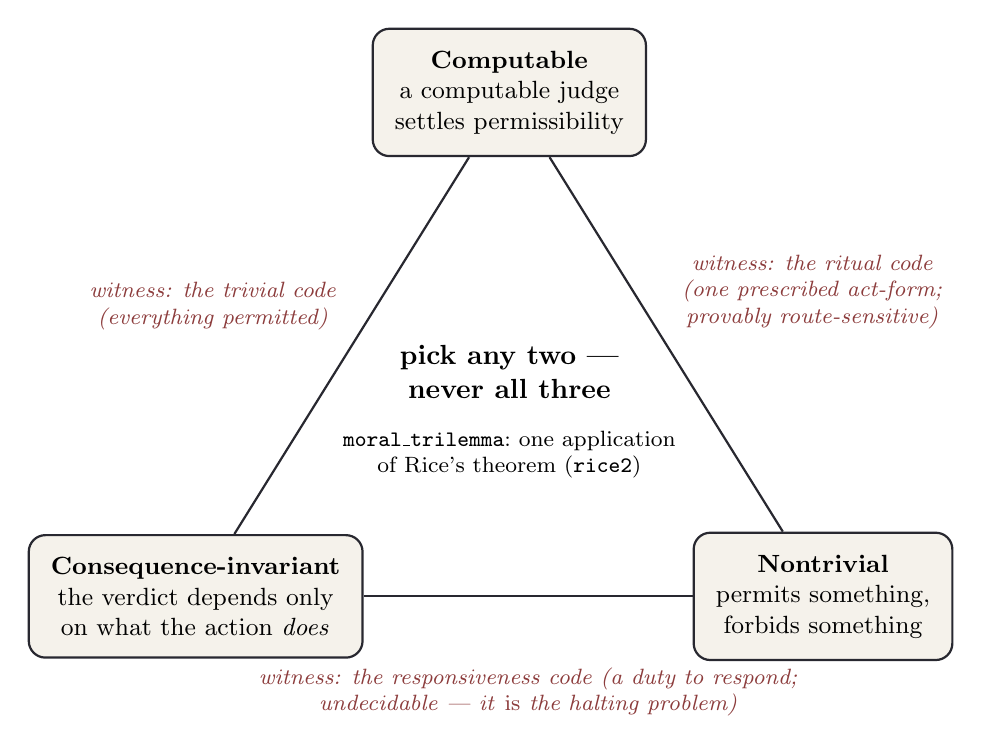
\begin{tikzpicture}[
  vertex/.style={draw=ink, thick, rounded corners=6pt, fill=soft,
    align=center, inner sep=8pt, font=\small},
  wit/.style={align=center, font=\footnotesize\itshape, text=accent},
  every path/.style={thick, draw=ink}
]
  % vertices of the triangle
  \node[vertex] (A) at (90:4.1)  {\textbf{Computable}\\a computable judge\\settles permissibility};
  \node[vertex] (B) at (210:4.6) {\textbf{Consequence-invariant}\\the verdict depends only\\on what the action \emph{does}};
  \node[vertex] (C) at (-30:4.6) {\textbf{Nontrivial}\\permits something,\\forbids something};

  % edges with pairwise witnesses
  \draw (A) -- (B) node[wit, midway, above left=2pt and 2pt]
    {witness: the trivial code\\(everything permitted)};
  \draw (A) -- (C) node[wit, midway, above right=2pt and 2pt]
    {witness: the ritual code\\(one prescribed act-form;\\provably route-sensitive)};
  \draw (B) -- (C) node[wit, midway, below=22pt]
    {witness: the responsiveness code (a duty to respond;\\undecidable --- it \emph{is} the halting problem)};

  % center
  \node[align=center, font=\bfseries] at (0,0.55)
    {pick any two ---\\never all three};
  \node[align=center, font=\footnotesize] at (0,-0.5)
    {\texttt{moral\_trilemma}:\ one application\\of Rice's theorem (\texttt{rice2})};
\end{tikzpicture}
\end{center}

\vspace{4pt}

{\small
\textbf{Setting.} Actions are programs (partial recursive codes); an
action's \emph{consequence profile} is the partial function it computes
over situations; a moral code is a set of permissible actions.
\textbf{Theorem.} No moral code is simultaneously computably judgeable,
consequence-invariant, and nontrivial. Every pair is jointly satisfiable,
witnessed as above. \textbf{Corollary} (\texttt{decidable\_nontrivial\_route\_sensitive}).
Decidability \emph{forces} route-sensitivity: a workable moral code must
distinguish some actions with identical consequences --- judging the act
rather than the outcome is not deontological taste but the only computable
option. \textbf{Moral halting theorem}
(\texttt{responsivenessCode\_undecidable}). The duty to determine whether
an action will respond cannot be computably audited.
}

\vspace{8pt}

\begin{center}
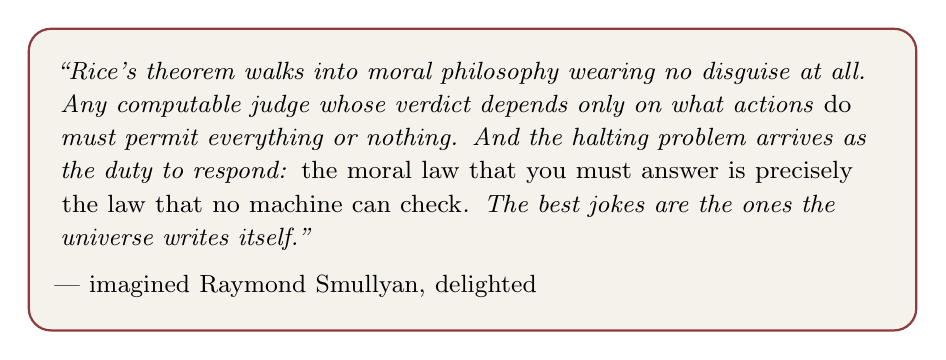
\begin{tikzpicture}
\node[draw=accent, thick, rounded corners=8pt, fill=soft, inner sep=12pt,
      text width=0.86\linewidth, align=left] {%
{\small\itshape ``Rice's theorem walks into moral philosophy wearing no
disguise at all. Any computable judge whose verdict depends only on what
actions \emph{do} must permit everything or nothing. And the halting
problem arrives as the duty to respond:
\emph{the moral law that you must answer is precisely the law that no
machine can check}. The best jokes are the ones the universe writes
itself.''}\\[5pt]
{\small --- imagined Raymond Smullyan, delighted}%
};
\end{tikzpicture}
\end{center}

\vfill

{\footnotesize
Verified in Lean~4 over Mathlib's computability library; no additional
axioms. Companion results: consequentializing, deontizing, and
virtualizing are each \emph{universal} at the price of a gerrymandered
presentation, and undecidability transfers along every faithful computable
translation between paradigms. Complexity-theoretic context: J.~Stenseke,
\emph{On the computational complexity of ethics}, AI Review (2024).
}

\end{document}
